
\begin{figure*}[t]
	\centering
	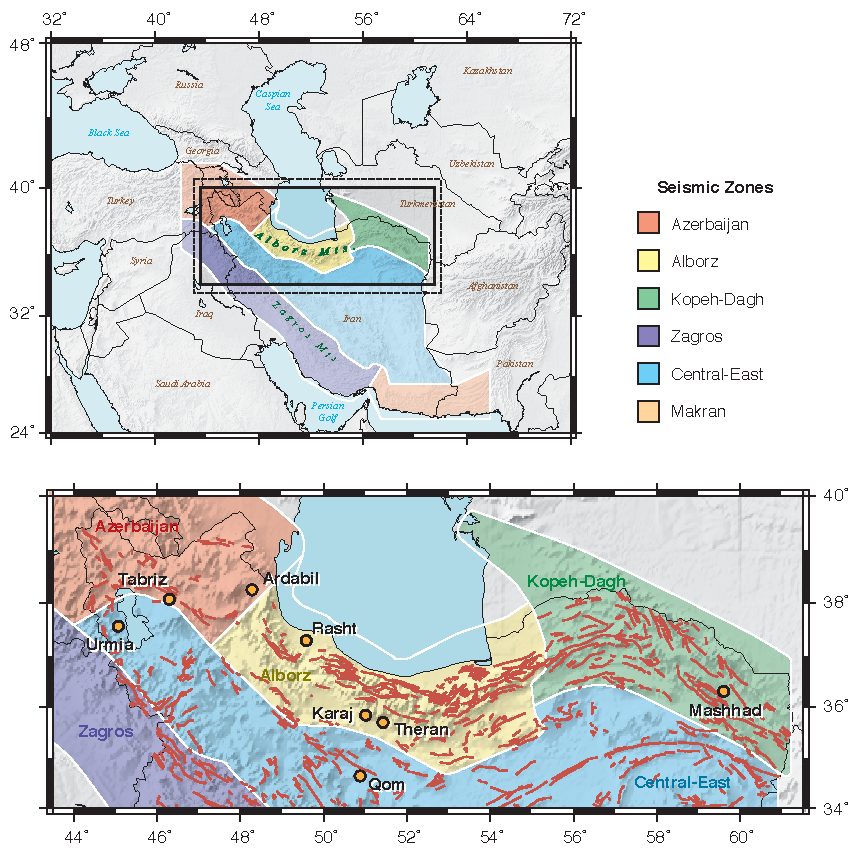
\includegraphics[width=0.9\textwidth]{figures/pdf/figure-01}
	\caption{Region of interest and Iranian seismic zones. At the top, the map of Iran and surrounding countries with shaded relief in the background and the Iranian seismic zones \citep[after][]{Karimiparidari2013} and region of interest in the foreground. The dashed box indicates the complete region of interest and the thicker line box indicates the effective area for which seismic hazard is estimated. The effective region of interest is shown in greater detail at the bottom. It includes the location of the major urban centers and seismic faults in northern Iran.}
	\label{fig:iran}
\end{figure*}

\begin{figure*}[t]
	\centering
	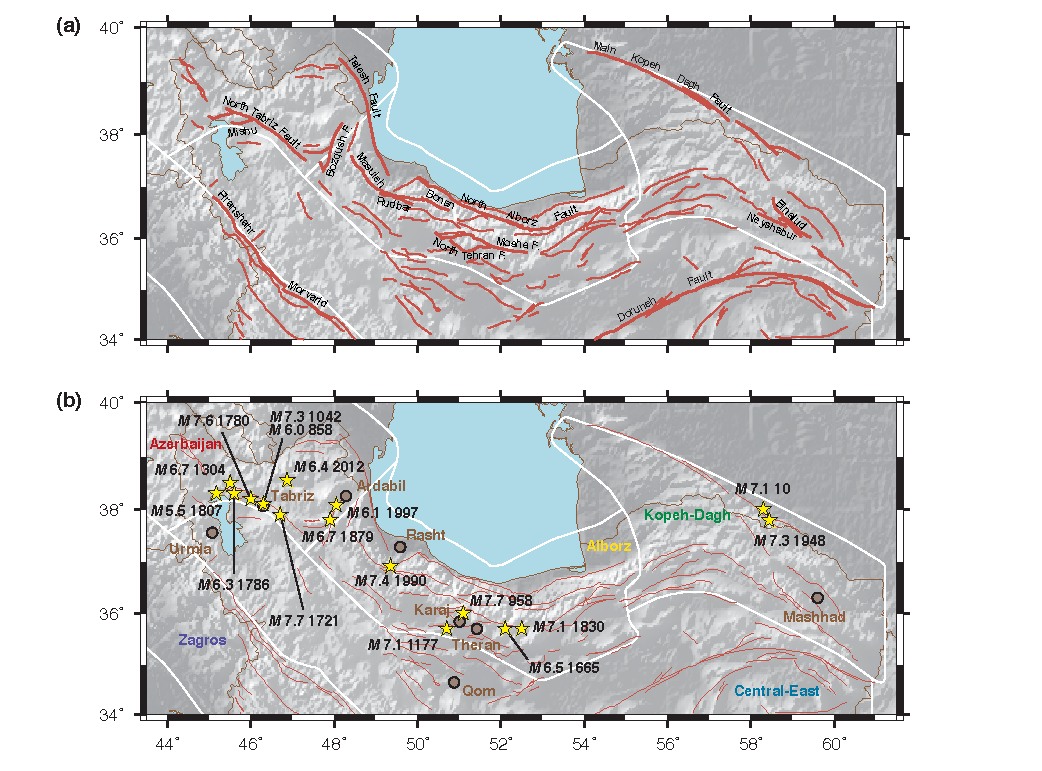
\includegraphics[width=0.9\textwidth]{figures/pdf/figure-02}
	\caption{(a) Main fault line and fault systems, and (b) notable earthquakes in the effective region of interest. White lines delimit the three major seismic zones in northern Iran. Epicentral locations are indicated with stars. The labels next to each star or linked with a line to avoid congestion show the magnitude and year of the earthquake. The borderlines of the seismic zones shown in Fig.~\ref{fig:iran} are shown in the background in white, along with the light gray shaded relief.}
	\label{fig:selected}
\end{figure*}

\section{Region of Interest}

We define our effective region of interest between longitudes 43.5\textdegree{}E and 61.5\textdegree{}E, and latitudes 34\textdegree{}N and 40\textdegree{}N, as shown in Fig.~\ref{fig:iran}. These limits correspond to the area for which we will present results in subsequent sections. Our calculations, however, included data from a larger region with a 2\textdegree{}-perimeter as indicated in the figure. This is done to avoid the artificial decay effect that results from smoothing the seismicity along and near the edges of the effective region of interest and/or to provide a uniform contribution from the earthquakes surrounding the region \citep[see][]{Lapajne1997}. The effective region has an area of 1,703 km $\times$ 667 km. It encloses the northern part of Iran with most of the Azerbaijan seismic zone, the complete zones of Alborz and Kopeh-Dagh, and the northernmost portions of the Zagros and Central-East seismic zones.

At the northwest of Iran, the seismic zone of Azerbaijan is strongly controlled by the North Tabriz Fault (NTF) system. This system, shown in Fig.~\ref{fig:selected}a, is a complex northwest-trending structure with a predominant right-lateral, strike-slip faulting mechanism \citep{Berberian1999}. Historical accounts document the occurrence of earthquakes in this area as far back as to the 9th century, with events in the years 858 ($M$ 6.0), 1042 ($M$ 7.3), and 1304 ($M$ 6.7) \citep{Berberian1999}. In the 18th century, in particular, the NTF ruptured three times in a span period of 65 years, which included the $M$ 7.7 1721 Tabriz earthquake in the southeastern section, the $M$ 7.6 1780 Tabriz earthquake in the northwestern section, and the $M$ 6.3 1786 Marand-Mishu on the Mishu reverse fault and the Sufian segment of the NTF. According to \citet{Jones1834}, the 1721 Tabriz earthquake had a surface rupture of more than 42 km and presented vertical separations of about 2 to 4 m. The locations of these and other notable events, including the $M$ 5.5 1807 Tasuj and the $M$ 6.7 1879 South Bozqush earthquakes, are shown in Fig.~\ref{fig:selected}b. More recently, the same region was struck by the $M_w$ 6.1 1997 Ardabil and $M_w$ 6.4 2012 Tabriz earthquakes, which caused extensive damage and took the lives of more than 1500 people.

Transitioning from the Azerbaijan to the Alborz seismic zone, the next fault system runs along the Rocks of the Talesh mountains, to the northwest of the Alborz Mountains. Faults in this area have also ruptured recently \citep{Berberian1999}. The $M_w$ 7.4 1990 Manjil-Rudbar earthquake, for instance, caused numerous deaths and significant damage to the region in the south Caspian depression. At the central area of the Alborz seismic zone, near Tehran, the region is characterized by active reverse faults in the North Tehran Thrust (NTT) system (see Fig.~\ref{fig:selected}a for reference). These faults are parallel to the northwest-trending structural gain of the Alborz Mountains belt, and include the south-dipping partially blind faults of Davudieh, Shian, and Bagh-E Feyz. According to \citet{Ambraseys_1982_Book}, Tehran---or the ancient city of Rey---has been devastated in multiple occasions due to severe earthquakes in this area. Historical accounts document the occurrence of multiple $M>7$ earthquakes in 743, 958, 1177, 1665, and 1830. The 1830 earthquake, in particular, ruptured the central segments of the NTT, adjacent to the Mosha fault.

To the east, the Main Kopeh-Dagh Fault is the predominant faulting system in the seismic zone with the same name. This system consists of several partly overlapping segments parallel to a NW--SE oriented structure of step-overs, which exhibits active tectonic displacements along a distance of more than 500 km \citep{Trifonov1978}. The system is also characterized by short south-dipping thrust faults striking E--W \citep{Berberian2001}. The Main Kopeh-Dagh Fault is responsible for the $M_w$ 7.3 1948 earthquake (Fig.~\ref{fig:selected}b). This event struck Ashgabat, the capital city of Turkmenistan, and destroyed more than 30 villages in Iran. Historically, the Kopeh-Dagh seismic zone is also responsible for multiple earthquakes at the boundary between the Neyshabur and Binalud reverse faults (Fig.~\ref{fig:selected}a) between 1209 and 1405 \citep{Berberian1999}, and an estimated $M_s$ 7.1 earthquake in 10 A.D.~\citep{Berberian2001}.
